\documentclass{beamer}
\usepackage{beamerthemesplit}
\usepackage{wrapfig}
\usetheme{SPbGU}
\usepackage{pdfpages}
\usepackage{amsmath}
\usepackage{mathtools}
\usepackage{cmap}
\usepackage[T2A]{fontenc}
\usepackage[utf8]{inputenc}
\usepackage[english,russian]{babel}
\usepackage{indentfirst}
\usepackage{amsmath}
\usepackage{tikz}
\usepackage{multirow}
\usepackage[noend]{algpseudocode}
\usepackage{algorithm}
\usepackage{algorithmicx}
\usepackage{ stmaryrd }
\usepackage{qtree}
\usetikzlibrary{shapes,arrows}
\usepackage{fancyvrb}
\usepackage{minted}
%\usepackage{forest}
%\usepackage{tikz-qtree}
%\usepackage{fontawesome}

\usetikzlibrary{calc}
\usetikzlibrary{shapes,arrows}
\usetikzlibrary{arrows,automata}
\usetikzlibrary{positioning}


\newtheorem{rutheorem}{Теорема}
\newtheorem{ruproof}{Доказательство}
\newtheorem{rudefinition}{Определение}
\newtheorem{rulemma}{Лемма}
\beamertemplatenavigationsymbolsempty

\setbeamertemplate{itemize item}[circle]
\setbeamertemplate{enumerate item}[circle]

\newcommand{\highlight}[2][yellow]{\mathchoice%
  {\colorbox{#1}{$\displaystyle#2$}}%
  {\colorbox{#1}{$\textstyle#2$}}%
  {\colorbox{#1}{$\scriptstyle#2$}}%
  {\colorbox{#1}{$\scriptscriptstyle#2$}}}%


\newcommand{\derive}[0]{\xRightarrow[]{*}}
\newcommand{\derives}[0]{\xRightarrow[]{}}
\newcommand{\derivek}[1]{\xRightarrow[]{#1}}
\newcommand{\deriveg}[1]{\xRightarrow[#1]{*}}
\newcommand{\derivegone}[1]{\xRightarrow[#1]{}}

\tikzset{
    state/.style={
           rectangle,
           rounded corners,
           draw=black, very thick,
           minimum height=2em,
           inner sep=2pt,
           text centered,
           },
}


\title[]{Теория автоматов и формальных языков}
\subtitle[]{Применение запросов с контекстно-свободными ограничениями для решения прикладных задач}
\institute[]{
Санкт-Петербургский государственный университет\\
}

\author[]{Григорьев Семён}

\date{17 декабря 2020}

\begin{document}
{
  \begin{frame}
    \titlepage
  \end{frame}
}

\begin{frame}[fragile]
  \frametitle{Пути с контекстно-свободными ограничениями (CFPQ)}
   \begin{itemize}
      \item Конечный ориентированный граф с метками на рёбрах $\mathcal{G} = (V,E,L)$
      \item Путь --- это слово в алфавите $L$ $\omega(p) = \omega(v_0 \xrightarrow{l_0} v_1 \xrightarrow{l_1} \dots \xrightarrow{l_{n-1}} v_n ) = l_0 \cdot l_1 \cdot \ldots \cdot l_{n-1}$
      \item $\mathcal{L}$ --- контекстно-свободный язык (КС язык)
      \item $G_{\mathcal{L}} = (N,\Sigma,R,S)$
    \end{itemize}
    \pause
    \begin{itemize}
      \item Задача достижимости: $Q=\{(v_i,v_j) \ | \ \exists p = v_i \dots v_j, S \xrightarrow[G_{\mathcal{L}}]{*} \omega(p) \}$
      \item Задача поиска путей: $Q=\{p \ | \ S \xrightarrow[G_{\mathcal{L}}]{*} \omega(p)\}$
      \begin{itemize}
        \item Один путь, все пути, кратчайший путь\dots
      \end{itemize}
    \end{itemize}

\end{frame}


\begin{frame}[fragile]
  \frametitle{Области применения CFPQ}
    \begin{itemize}
      \item Статический анализ кода
      \begin{itemize}
        \item Межпроцедурный анализ указателей
        \item Анализ типов
        \item Унификация
        \item ...
      \end{itemize}
      \item Анализ биологических данных
      \item Обработка грвф-структурированных данных (графовые базы данных)
  \end{itemize}
\end{frame}

\begin{frame}[fragile]
  \frametitle{Пример (База данных)}
  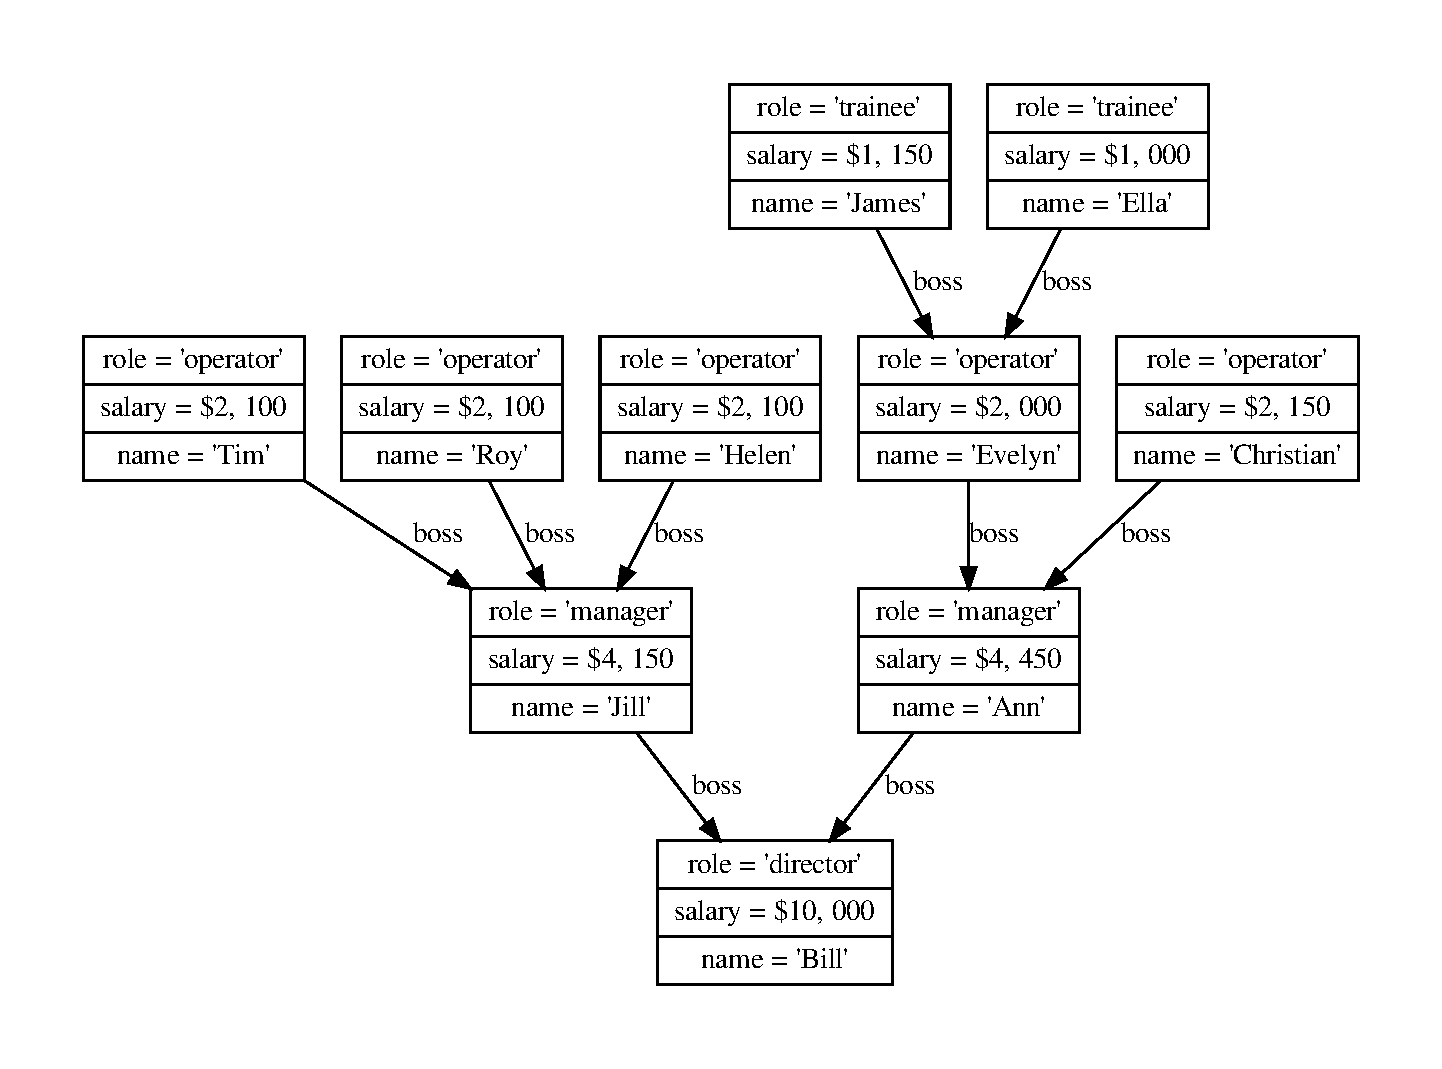
\includegraphics[width=0.95\textwidth]{figures/cfpq_example.pdf}
\end{frame}


\begin{frame}[fragile]
  \frametitle{Пример (Запросы)}
  \begin{itemize}
  \item Найти всех, занимающих одинаковое положение в структуре организации, но имеющих разные зарпллаты (на Cypher)
    \begin{minted}{plpgsql}
PATH PATTERN OnSamePosition  =
  ()-/ :boss> [~OnSamePosition | ()] <:boss /->()
MATCH (a)-/ ~OnSamePosition /->(b)
WHERE a.salary <> b.salary
RETURN a, b
    \end{minted}
\pause
  \item Кто в структуре ниже Тима, но имеет более высокую зарплату
    \begin{minted}{plpgsql}
PATH PATTERN OnSamePosition  =
  ()-/ :boss> [~OnSamePosition | ()] <:boss /->()
MATCH
  (a:{name: 'Tim'})-/ ~OnSamePosition /-> ()
   <-[boss*1..]- (b)
WHERE a.salary < b.salary
RETURN b
    \end{minted}

\end{itemize}

\end{frame}

\begin{frame}[fragile]

  \frametitle{Статический анализ кода}

Межпроцедурный анализ кода
\begin{itemize}
\item \emph{Thomas Reps et al.} ``Precise interprocedural dataflow analysis via graph reachability.'' 1995
\pause
\item \emph{Qirun Zhang et al.}  ``Efficient subcubic alias analysis for C.'' 2014
\item \emph{Dacong Yan et al.} ``Demand-driven context-sensitive alias analysis for Java.'' 2011
\pause
\item \emph{Anders Alnor Mathiasen, and Andreas Pavlogiannis.} ``The Fine-Grained and Parallel Complexity of Andersen’s Pointer Analysis.`` 2020 (POPL 2021)
\end{itemize}

\end{frame}

\begin{frame}[fragile]

  \frametitle{Пример}
  \begin{columns}[c] % The "c" option specifies centered vertical alignment while the "t" option is used for top vertical alignment

\column{.25\textwidth} % Left column and width
 \begin{minted}{java}
  v.h = u;
  ...
  p = v;
  ...
  q.g = p;
  ...
  w = q;
  ...
  x = w.g;
  if (...) {
    y = w.f;
  }
  else {
    y = x.h;
  }
\end{minted}

\column{.6\textwidth} % Right column and width
\begin{figure}[h]
    \centering
    \begin{tikzpicture}[shorten >=1pt,auto]
       \node[state] (q_0)                      {$u$};
       \node[state] (q_1) [right=of q_0] {$v$};
       \node[state] (q_2)  [above=of q_1]  {$p$};
       \node[state] (q_3) [right=of q_2] {$q$};
     \node[state] (q_4) [below=of q_3] {$w$};
     \node[state] (q_5) [right=of q_4] {$x$};
    \node[state] (q_6) [below=of q_5] {$y$};

        \path[->]
        (q_0) edge  node {$h$} (q_1)
        (q_1) edge[thick]  node {$$} (q_2)
        (q_2) edge  node {$g$} (q_3)
       (q_3) edge [thick] node {$$} (q_4)
       (q_4) edge  node {$\bar{g}$} (q_5)
      (q_5) edge  node {$\bar{h}$} (q_6)
       (q_4) edge[bend right, below]  node {$\bar{f}$} (q_6);

    \end{tikzpicture}
\end{figure}
Correct path: \textcolor{green}{$hg\bar{g}\bar{h}$}

Incorrect path: \textcolor{red}{$hg\bar{f}$}

\end{columns}

\end{frame}

\begin{frame}[fragile]

  \frametitle{Пара слов о практической применимости}
  \begin{itemize}
\item Interprocedural static nullability analysis\footnote{\emph{Kai Wang et. al.} Graspan: a single-machine disk-based graph system for interprocedural static analyses of large-scale systems code. 2017}

\begin{itemize}
   \item ``We have identified a total of 1127 unnecessary NULL tests in Linux, 149 in PostgreSQL,
   32 in httpd.''
   \item ``Our analyses reported 108 new NULL pointer dereference bugs in Linux, among which 23 are false positives''
   \item ``For PostgreSQL and httpd, we detected 33 and 14 new NULL pointer bugs; our manual validation did not find any false positives among them.''
\end{itemize}

\end{itemize}

\end{frame}


\begin{frame}[fragile]

  \frametitle{Другие задачи анализа кода}
  \begin{itemize}
    \item \emph{Yulei Sui, et al.} ``Flow2Vec: value-flow-based precise code embedding.'' 2020
    \pause
    \item \emph{Osbert Bastani, Saswat Anand, and Alex Aiken.} ``Specification inference using context-free language reachability.'' 2015
    \item \emph{Jakob Rehof and Manuel Fahndrich.} ``Type-base flow analysis: from polymorphic subtyping to CFL-reachability.'' 2001
    \pause
    \item \emph{Das, Manuvir, and Thomas Reps.} ``BTA termination using CFL-reachability.'' 1996\footnote{Доклад на семинаре: \url{https://vk.com/ycformallanguagesseminar?w=wall-154415012_63}}
    \pause
    \item \emph{Venkatesh Choppella, and Christopher T. Haynes.} ''Source-tracking unification.'' 2005\footnote{Доклад на семинаре: \url{https://vk.com/ycformallanguagesseminar?w=wall-154415012_94}}
  \end{itemize}

\end{frame}

\begin{frame}[fragile]

  \frametitle{За пределами КС граммтик}
  \begin{itemize}
      \item Пусть $L_1 = D_1(\textit{deref}, \textit{ref}) $  \ и \ $ L_2 = D_1(\textit{call}, \textit{return})$
      \item Язык ограничений $L_3 = L_1 \odot L_2 = \{\textit{call return}; \textit{call deref return deref ref ref};  \dots\}$ --- шафл сбалансированных скобочных последовательностей
      \item $L_3$ не является контекстно-свободным, но является линейно-конъюктивным
    \end{itemize}

\end{frame}

\begin{frame}[fragile]

  \frametitle{Исследования линейно-конъюнктивных ограничений}
  \begin{itemize}
      \item \emph{Qirun Zhang and Zhendong Su.} ``Context-sensitive data-dependence analysis via linear conjunctive language reachability.'' 2017
      \item \emph{Yuanbo Li, Qirun Zhang, and Thomas Reps.} ``Fast graph simplification for interleaved Dyck-reachability.'' 2020.
    \end{itemize}

\end{frame}


\begin{frame}[fragile]

  \frametitle{Графовые базы данных}
  \begin{itemize}
    \item \emph{Mihalis Yannakakis.} ``Graph-theoretic methods in database theory.'' 1990
    \item \emph{Hellings J.} ``Conjunctive context-free path queries.'' 2014
    \item \emph{J. Kuijpers, G. Fletcher, N. Yakovets, and T. Lindaaker.} ``An experimental
study of context-free path query evaluation methods.'' 2019
    \item \emph{C. M. Medeiros, M. A. Musicante, and U. S. Costa.} ``LL-based query answering
over rdf databases.'' 2019
  \end{itemize}
\end{frame}

\begin{frame}[fragile]

  \frametitle{Анализ биологических данных\footnote{\emph{Sevon P., Eronen L.} ``Subgraph queries by context-free grammars.'' 2008}}
  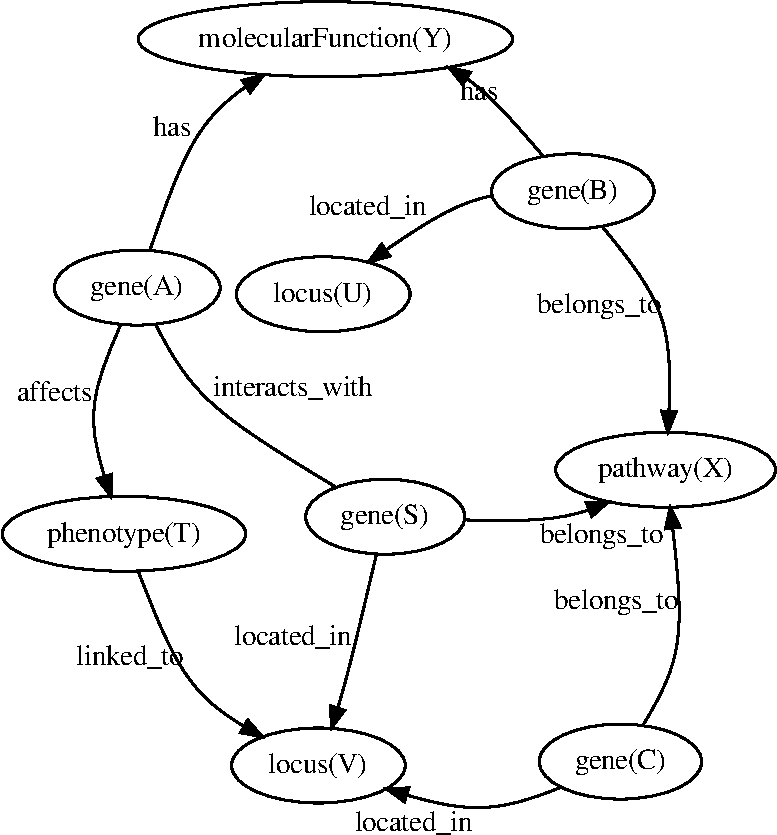
\includegraphics[width=0.55\textwidth]{figures/bioDB-crop.pdf}
\end{frame}

\begin{frame}[fragile]

  \frametitle{Анализ биологических данных (запрос)}
    \begin{minted}{ocaml}
IS_ASSOCIATED_TO -> -refers_to ARTICLE refers_to

SEQUENCE -> GENE
          | PROTEIN
          | GENE codes_for PROTEIN
          | PROTEIN -codes_for GENE

GENE -> GENE IS_SIMILAR_TO gene | gene
PROTEIN -> PROTEIN IS_SIMILAR_TO protein | protein
PHENOTYPE -> PHENOTYPE IS_SIMILAR_TO phenotype | phenotype

(*for all (edge symbol, vertex non-terminal)-pairs (e, V),
and for all similarity-conferring edge types 'h'
(e.g., is_homologous_to) *)
V -> V IS_SIMILAR_TO v | v
IS_SIMILAR_TO -> e V -e | h
    \end{minted}

\end{frame}

\begin{frame}[fragile]

  \frametitle{Анализ биологических данных (запрос)}
    \begin{minted}{ocaml}
FROM protein("ACHB3_HUMAN")
TO phenotype("AD")
MATCH SEQUENCE IS_ASSOCIATED_TO PHENOTYPE
    \end{minted}

\end{frame}


\end{document}
